Tras establecer los parámetros necesarios correspondientes a la gestión del proyecto, este capítulo presenta el diseño del sistema implementado. Para ello se introducirá la estructura de directorios utilizada, el diagrama del software desarrollado y la gestión de las herramientas con el protocolo MCP. 

\section{Estructura del proyecto}
El repositorio se estructura en cuatro componentes independientes, cada uno con su propio entorno virtual de Python (venv\footnote{venv: \url{https://docs.python.org/3/library/venv.html}}). La Figura \ref{fig:dir_principales} ilustra la organización jerárquica de los directorios principales.

\begin{figure}[p]
\centering
\definecolor{folderbg}{RGB}{124,166,198}
\definecolor{folderborder}{RGB}{110,144,169}
\newlength\Size
\setlength\Size{4pt}
\tikzset{%
  folder/.pic={%
    \filldraw [draw=folderborder, top color=folderbg!50, bottom color=folderbg] (-1.05*\Size,0.2\Size+5pt) rectangle ++(.75*\Size,-0.2\Size-5pt);
    \filldraw [draw=folderborder, top color=folderbg!50, bottom color=folderbg] (-1.15*\Size,-\Size) rectangle (1.15*\Size,\Size);
  },
  file/.pic={%
    \filldraw [draw=folderborder, top color=folderbg!5, bottom color=folderbg!10] (-\Size,.4*\Size+5pt) coordinate (a) |- (\Size,-1.2*\Size) coordinate (b) -- ++(0,1.6*\Size) coordinate (c) -- ++(-5pt,5pt) coordinate (d) -- cycle (d) |- (c) ;
  },
}
\forestset{%
  declare autowrapped toks={pic me}{},
  declare boolean register={pic root},
  pic root=0,
  pic dir tree/.style={%
    for tree={%
      folder,
      font=\ttfamily,
      grow'=0,
      % Reducción del espaciado vertical entre nodos
      s sep=0.12cm,
      % Reducción del espaciado horizontal entre niveles
      l sep=0.8cm,
    },
    before typesetting nodes={%
      for tree={%
        edge label+/.option={pic me},
      },
      if pic root={
        tikz+={
          \pic at ([xshift=\Size].west) {folder};
        },
        align={l}
      }{},
    },
  },
  pic me set/.code n args=2{%
    \forestset{%
      #1/.style={%
        inner xsep=2\Size,
        pic me={pic {#2}},
      }
    }
  },
  pic me set={directory}{folder},
  pic me set={file}{file},
}
\begin{forest}
  pic dir tree,
  pic root,
  for tree={% folder icons by default; override using file for file icons
    directory,
  },
  [tfg\_agentes\_software
    [servidor\_mcp\_bd\_codigo
    [src
    [mcp\_code\_server.py, file]
    ]
    ]
    [servidor\_mcp\_confluence
    [launch\_mcp\_server\_confluence.py, file]
    ]
    [servidor\_mcp\_google\_drive
    [credentials]
    [index\_mod.js, file]
    ]
    [sistema\_agentes
    [src
    [db]
    [evaluators]
    [formatter\_agent]
    [orchestrator\_agent]
    [planner\_agent]
    [specialized\_agents
    [citation\_tools]
    [confluence\_agent]
    [filesystem\_agent]
    [gitlab\_agent]
    [google\_drive\_agent]
    [SpecializedAgent.py, file]
    ]
    [BaseAgent.py, file]
    [main\_graph.py, file]
    [structured\_output\_validator.py, file]
    [utils.py, file]
    ]
    [static
    [gen\_docs
    ]
    [agent\_descriptions.py, file]
    [prompts.py, file]
    ]
    [main.py, file]
    [config.py, file]
    [.env, file]
    ]
  ]
\end{forest}
\caption{Estructura de directorios principales del proyecto}
\label{fig:dir_principales}
\end{figure}

El directorio \texttt{sistema\_agentes} alberga todos los agentes desarrollados junto con los clientes MCP. La implementación de los agentes se ubica en el directorio \texttt{src}, mientras que \texttt{static} contiene los prompts utilizados, las descripciones de los agentes y la documentación oficial generada. El archivo \texttt{.env} almacena variables secretas como las claves de acceso a APIs, y el archivo \texttt{config.py} gestiona variables globales como el modelo predeterminado utilizado en los agentes. El archivo \texttt{main.py} integra la lógica de ejecución principal, mientras que \texttt{src/main\_graph.py} implementa el agente Main.

Los directorios \texttt{servidor\_mcp\_bd\_codigo}, \texttt{servidor\_mcp\_confluence} y \texttt{servidor\_mcp\_google\_drive} contienen cada uno un servidor MCP de ejecución independiente. 
\section{Diseño de agentes}

LangGraph proporciona un marco de trabajo estructurado para la creación de flujos de ejecución en forma de grafo. Se construye inicialmente un grafo mediante el objeto StateGraph\todo{Debería referenciar en el pie de página la documentación de las clases de las librerías que menciono? Me ha dicho Claude que sobrecargaría demasiado la memoria.}, el cual establece la lógica de enrutamiento entre diversos nodos definidos como funciones de Python. Estos grafos utilizan un denominado estado, representado por un diccionario tipado, para almacenar el estado de ejecución durante el proceso.

Bajo este paradigma, un agente puede representarse como un grafo compilado, donde uno o varios nodos definen la lógica de invocación a los modelos LLM, mientras que otros nodos se encargan de interpretar el resultado. En una implementación tradicional, el estado conservaría los mensajes generados entre llamadas, lo que posibilita un proceso iterativo en el cual el nodo de invocación al LLM se ejecuta repetidamente, añadiendo un nuevo mensaje al estado en cada ciclo de ejecución.
\todo{Estos dos párrafos quizás quedarían mejor en una breve sección en antecedentes?}

Este enfoque proporciona un marco de trabajo orientado a la composición, puesto que un nodo puede constituir a su vez otro grafo compilado que represente a otro agente. Sin embargo, presenta una problemática de redundancia: cuando dos agentes comparten gran parte del grafo que los compone, para evitar la duplicación de código sería necesario desarrollar un grafo que contemple la ejecución de ambos tipos de agentes, determinando en cada instancia cuál ejecutar en función de un parámetro presente en el estado. Aunque esta solución es viable, la programación orientada a objetos ofrece una alternativa más elegante: la herencia.

Es por este motivo que se ha optado por un enfoque híbrido que combina composición y herencia. Cada agente está implementado mediante una clase de Python, la cual contiene la función \texttt{create\_graph()}, que compone el grafo representativo de la ejecución del agente. De esta manera, la clase del agente define las funciones que representan cada nodo del grafo, pudiendo heredar aquellas definidas en clases más abstractas.

Adicionalmente, esta metodología facilita el almacenamiento de datos no vinculados a la ejecución individual. Los datos encapsulados en los atributos de las clases representan información invariable en cada ejemplo de ejecución, como el nombre del agente o las herramientas disponibles; mientras que los atributos almacenados en el estado del grafo son específicos de la ejecución, como los mensajes generados durante la instancia de ejecución concreta.

\subsection{Diagrama de agentes}

\begin{figure}[p]
  \centering
  \adjustbox{center=\textwidth}{\hspace{-1.2cm}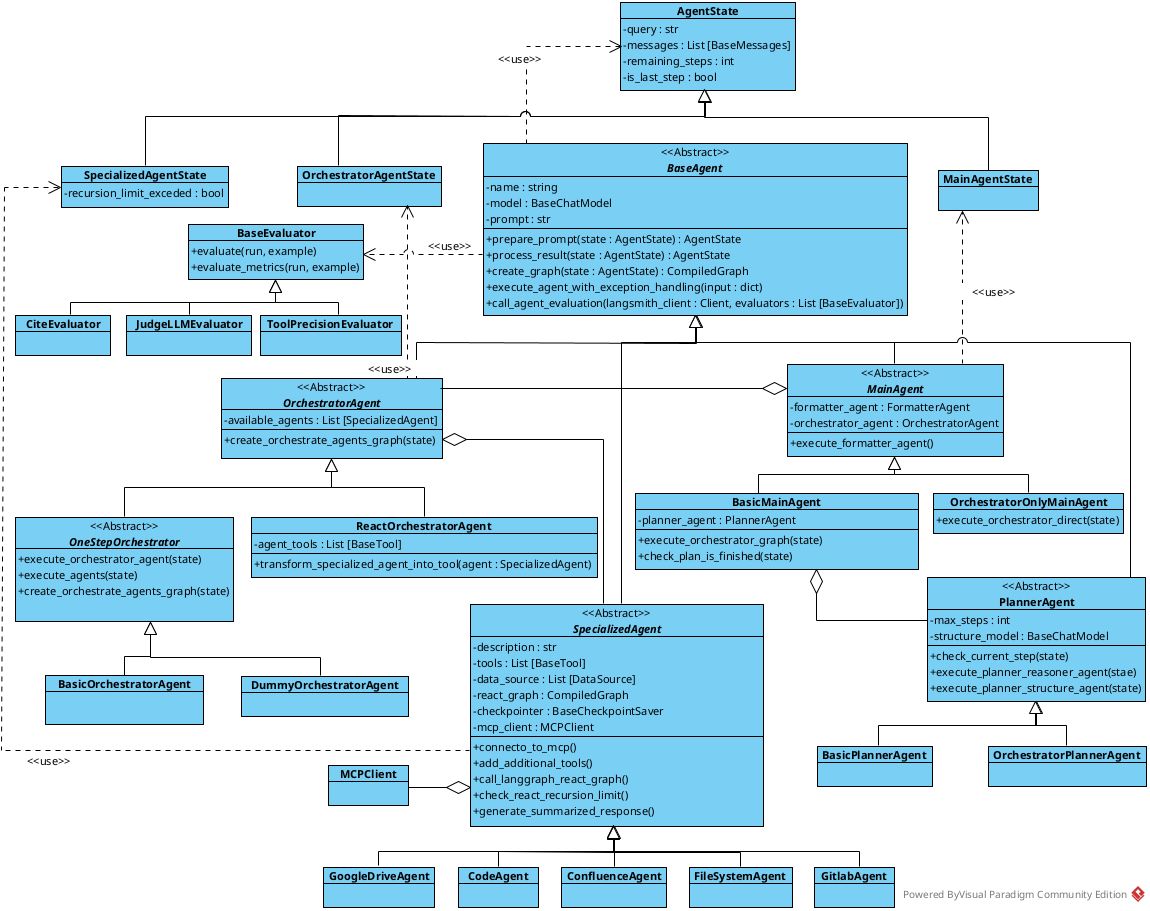
\includegraphics[width=1.4\linewidth]{figures/agentes.png}}
  \caption{Diagrama de clases UML de del sistema de agentes.}
  \label{fig:uml}
\end{figure}

La Figura \ref{fig:uml} ilustra el diagrama de clases (UML) general del sistema, donde se puede observar que la clase abstracta \texttt{BaseAgent} constituye la base del que heredan todos los agentes. Dicha clase establece las funcionalidades comunes que implementan todos los agentes del sistema:

\begin{itemize}
\item \textbf{Lógica de ejecución:} la función \texttt{execute\_agent\_with\_exception\_handling()} se encarga de invocar el grafo definido en la función \texttt{create\_graph()}, gestionando las posibles excepciones e inicializando los parámetros de entrada requeridos. Todos los agentes derivados deben implementar la función \texttt{prepare\_prompt()} e integrarla en su grafo de ejecución correspondiente, para definir el mensaje inicial del sistema que instruye al agente.
\item \textbf{Gestión del resultado:} La función \texttt{process\_result()} se encarga de procesar y devolver de manera estática el resultado de ejecución del agente para un estado de ejecución determinado. Dependiendo del agente concreto, este resultado puede comprender todos los mensajes que satisfagan determinados criterios establecidos.
\item \textbf{Evaluación del agente:} La función \texttt{call\_agent\_evaluation()} establece la lógica de evaluación específica para cada agente, utilizando las métricas definidas y representadas por la clase \texttt{BaseEvaluator}. El Capítulo \colorbox{yellow}{\ref{}} describe este proceso en detalle.
\end{itemize}

Los agentes que heredan del agente base son los siguientes:
\begin{itemize}
  \item \textbf{SpecializedAgent:} Representa de forma abstracta los agentes que realizan búsquedas en fuentes de información especializadas, aspecto detallado en la Sección \colorbox{yellow}{\ref{:west}}. Define la lógica de gestión de las herramientas utilizadas mediante el cliente MCP, utilizando la clase Singleton \texttt{MCPClient}, la cual encapsula la lógica de conexión con todos los servidores MCP disponibles, explicado en la Sección \ref{sec:gestionmcp}. Asimismo, contiene una secuencia de instancias de \texttt{DataSource}, las cuales definen todos los documentos citables en las fuentes de datos disponibles, descrito en la Sección \colorbox{yellow}{\ref{}}.
  \item \textbf{OrchestratorAgent:} Implementa la lógica de enrutamiento de los agentes especialistas, determinando en cada caso qué agentes ejecutar para resolver una cuestión específica. Véase la Sección \colorbox{yellow}{\ref{sec}}.
  \item \textbf{PlannerAgent:} Define la estrategia de planificación a seguir para una consulta determinada, elaborando planes secuenciales dinámicamente adaptables. Este proceso se detalla en la Sección \colorbox{yellow}{\ref{sec}}.
  \item \textbf{FormatterAgent:} Transforma una secuencia de ejecución de agentes en un resultado estructurado y comprensible, compuesto por una respuesta en formato textual y un conjunto de citas que referencian a documentos del proyecto software. Consulte la Sección \colorbox{yellow}{\ref{sec}}.
  \item \textbf{MainAgent:} Establece el flujo general de la ejecución, especificando si se implementarán agentes planificadores, orquestadores y enlanzando su respuesta al agente formateador. Este proceso se describe en la Sección \colorbox{yellow}{\ref{sec}}.
\end{itemize}

Cada agente implementa su propia clase de estado para gestionar los atributos vinculados a una ejecución específica, extendiendo la clase común \texttt{AgentState} que incorpora atributos como los mensajes a incluir en el contexto de entrada. Como se ha descrito en la Sección \ref{sec:abst}, la interacción con los agentes sigue una estructura conversacional. Para implementar esta estructura, se utilizan mensajes de LangChain: \texttt{SystemMessage} para las instrucciones que instruyen al agente, \texttt{HumanMessage} para las consultas o mensajes del usuario, y \texttt{AIMessage} para incorporar comunicaciones de agentes precedentes en el contexto de entrada.

Durante la fase de inicialización, se procede a la creación de los grafos correspondientes a todos los agentes mediante la instanciación de sus respectivas clases, estableciendo simultáneamente las conexiones necesarias con los servidores MCP. Una vez completado este proceso de inicialización, los agentes adquieren la capacidad de responder a todas las consultas requeridas sin necesidad de desconexión. 

\section{Servidores MCP utilizados}
En esta sección se describirán los cinco servidores MCP implementados, los cuales exponen sus herramientas mediante dos protocolos de comunicación introducidos en la Sección \ref{sec:mcp_prots}: el protocolo SSE (Server-Sent Events) y el protocolo STDIO (Standard Input/Output).

\subsection{Servidores SSE}
Estos se alojan en componentes separados, ya que el protocolo SSE permite desacoplar servidores y cliente MCP.

\begin{itemize}
  \item \textbf{Servidor Confluence:} proporciona acceso de lectura al repositorio Confluence, utilizando el servidor MCP oficial de Atlassian\footnote{Repositorio de servidor MCP Atlassian: \url{https://github.com/sooperset/mcp-atlassian}}. El componente \texttt{servidor\_mcp\_confluence} incorpora un script de lanzamiento \texttt{launch\_mcp\_server\_confluence.py} (detallado en el listado \ref{lst:servconf}), un entorno virtual \texttt{.venv} y un archivo \texttt{.env} destinado al almacenamiento de credenciales de Confluence.

    El script inicializa el servidor mediante el gestor de paquetes uv\footnote{Comando uvx: \url{https://docs.astral.sh/uv/guides/tools/}}, implementando el paquete mcp-atlassian\footnote{Paquete mcp-atlassian: \url{https://pypi.org/project/mcp-atlassian/}} disponible en PyPI\footnote{PyPI: \url{https://pypi.org/}}. Atlassian integra el Kit de desarrollo de software (SDK) del protocolo MCP\footnote{SDKs del protocolo MCP: \url{https://github.com/modelcontextprotocol}} en este paquete para desarrollar un servidor de Interfaz de Pasarela de Servidor Asíncrona (ASGI) con capacidades de enrutamiento de herramientas que interactúan con su API. Tras la extracción de variables de entorno desde \texttt{.env}, la biblioteca \texttt{subprocess}\footnote{Librería subprocess: \url{https://docs.python.org/3/library/subprocess.html}} ejecuta el comando uvx en el sistema, requiriendo que uvx esté previamente instalado en el entorno virtual.
\begin{lstlisting}[caption={\texttt{launch\_mcp\_server\_confluence.py}: ejecución de lanzamiento del servidor MCP Confluence},label={lst:servconf}]
    # Obtener variables de entorno
    load_dotenv() # <- Carga las variables desde el fichero .env
    confluence_url = os.getenv('CONFLUENCE_URL')
    ...

    # Construir el comando para uvx
    command = ["uvx", "mcp-atlassian"]
    
    command.extend(["--transport", mcp_transport])
    command.extend(["--port", mcp_port]) 
    command.extend(["--confluence-url", confluence_url])
    command.extend(["--confluence-username", confluence_username])
    command.extend(["--confluence-token", confluence_token])

    # Ejecutar el comando
    try:
        subprocess.run(command)
    ...
\end{lstlisting}

\item\textbf{Servidor Código: }proporciona acceso de lectura al repositorio software, implementando herramientas para la consulta de su código fuente. Su desarrollo se ha realizado directamente mediante el SDK de MCP para Python\footnote{SDK de MCP para Python: \url{https://github.com/modelcontextprotocol/python-sdk}}, localizado en el fichero \texttt{src/mcp\_code\_server.py} del componente \texttt{servidor\_mcp\_bd\_codigo}. La Sección \colorbox{yellow}{\ref{sec}} detalla la implementación de dichas herramientas.

  El sistema emplea la clase FastMCP, que integra internamente un servidor ASGI mediante la librería Starlette\footnote{Librería Starlette: \url{https://www.starlette.io/}} para gestionar el enrutamiento de las herramientas implementadas. Como se especifica en el Listado \ref{lst:mcpcod}, el procedimiento consta de la instanciación de la clase, la asociación de diversas herramientas mediante el decorador \texttt{mcp.tool}, y la posterior ejecución del servidor. Una vez vinculadas las herramientas, se generan automáticamente las rutas \texttt{call\_tool} y \texttt{get\_tools}, facilitando su acceso desde el cliente MCP.

\begin{lstlisting}[caption={\texttt{mcp\_code\_server.py: ejecución del servidor MCP con acceso al código fuente}},label={lst:mcpcod}]
  # Instanciar clase 
  mcp = FastMCP("postgre")

  # Vincular herramientas al servidor
  @mcp.tool()
  async def get_all_respository_files_list() -> TextContent:
      """
      Devuelve una lista en formato string serializable a JSON de todos los ficheros en el repositorio respecto a su ruta relativa
      """
      files_list = get_all_files_list(db_session=db_session)
      files_list_str=str(files_list)
      return TextContent(
          text=files_list_str,
          type='text'
      )

  # Ejecutar servidor
  if __name__ == "__main__":
      try:
          mcp.run(transport='sse')
       ...

\end{lstlisting}


\end{itemize}

\subsection{Servidores STDIO}
\label{sec:stdio}
Estos servidores se ejecutan estableciendo una conexión en el cliente MCP mediante una instancia de StdioServerParameters, que especifica los parámetros de configuración necesarios. De esta manera, cuando el cliente inicia la conexión, el servidor se ejecuta en un subproceso del mismo.

En los tres servidores la configuración de dicha instancia sigue el mismo procedimiento ilustrado en el Listado \ref{lst:mcpgitlab}. Se construye el comando con los argumentos correspondientes, se obtienen los argumentos a especificar en el comando y se incorporan las credenciales como variables de entorno.

\begin{lstlisting}[caption={mcp\_multi\_client.py: instanciado de StdioServerParameters para el servidor MCP de GitLab},label={lst:mcpgitlab}]
  # Crear comando y argumentos
  server_command = "npx"
  server_args = ["-y", "@modelcontextprotocol/server-gitlab"]

  # Obtener las credenciales desde las variables de entorno
  server_env = {
      "GITLAB_PERSONAL_ACCESS_TOKEN": os.getenv('GITLAB_PERSONAL_ACCESS_TOKEN'),
      "GITLAB_API_URL": GITLAB_API_URL
  }

  # Crear instancia StdioServerParameters indicando las credenciales de GitLab como variables de entorno
  server_params = StdioServerParameters(
      command=server_command,
      args=server_args,
      env=server_env
  )
  
\end{lstlisting}
Mediante este procedimiento, se han utilizado los siguientes servidores:
\begin{itemize}
  \item\textbf{Servidor Sistema de ficheros local: }Proporciona acceso a un directorio específico, que simula el repositorio de la ``documentación oficial'' del proyecto. Se ha utilizado el servidor de Anthropic FileSystem\footnote{FileSystem: \url{https://github.com/modelcontextprotocol/servers/tree/main/src/filesystem}}, ejecutándolo mediante el comando npx con el paquete del registro npm\footnote{npm: \url{https://www.npmjs.com/}} \texttt{@modelcontextprotocol/server-filesystem}\footnote{server-filesystem: \url{https://www.npmjs.com/package/@modelcontextprotocol/server-filesystem}}.

  \item\textbf{Servidor GitLab: }Facilita el acceso al repositorio de GitLab con funcionalidades para leer o modificar ficheros, incidencias, usuarios y contribuciones. Se ejecuta utilizando el paquete npm \texttt{@modelcontextprotocol/server-gitlab}\footnote{server-gitlab: \url{https://www.npmjs.com/package/@modelcontextprotocol/server-gitlab}}. Debido a que no ofrece capacidades específicas para la lectura de ciertos recursos (limitándose a operaciones de escritura), se han incorporado herramientas complementarias mediante la función \texttt{add\_additional\_tools()} en el agente \texttt{SpecializedAgent}, como se detalla en la Sección \colorbox{yellow}{\ref{sec:}}.

  \item\textbf{Servidor Google Drive: }Proporciona acceso a un directorio de Google Drive, donde se alojan las maquetas HTML del proyecto software. A pesar de existir un repositorio oficial de MCP para la conexión con Google Drive, este no ofrece todas las funcionalidades requeridas, por lo que se ha empleado una modificación desarrollada en JavaScript\footnote{Servidor MCP Google Drive: \url{https://github.com/felores/gdrive-mcp-server/blob/main/index.ts}}. En consecuencia, en lugar de especificar el paquete a utilizar en la instancia StdioServerParameters, se indica la ruta del script a ejecutar, como se muestra en el Listado \ref{lst:clientgd}.

\begin{lstlisting}[caption={mcp\_multi\_client.py: StdioServerParameters para el servidor MCP de Google Drive},label={lst:clientgd}]
  # Construir el comando indicando el script a ejecutar
  server_script_path = f"{server_path}/index_mod.js"
  server_command = "node"
  server_args = [server_script_path]

  server_params = StdioServerParameters(
      command=server_command,
      args=server_args,
      env=env
  )
\end{lstlisting}


Adicionalmente, se ha modificado la herramienta de listar ficheros para mostrar recursivamente todos los ficheros dentro de los directorios listados como se muestra en el Listado \ref{lst:mcpgd}


\begin{lstlisting}[caption={index\_mod.js: herramienta gdrive\_list\_files utilizando la API de Google Drive},label={lst:mcpgd}]
  // Utilizar librería de google drive para interactuar con la api
  import { google } from "googleapis";
  const drive = google.drive("v3"); 

  // Consultar archivos en la carpeta actual
  const res = await drive.files.list({
      q: `'${folderId}' in parents`,
      pageSize: 1000,
      fields: "files(id, name, mimeType, modifiedTime, size)"
  \});

  // Procesar cada archivo/carpeta
  for (const file of res.data.files || []) {
      allFiles.push({
        ...
      });
      
      // Si es una carpeta, listar su contenido recursivamente
      if (file.mimeType === 'application/vnd.google-apps.folder') {
          const subFiles = await listFilesRecursively(file.id, depth + 1, maxDepth);
          allFiles = allFiles.concat(subFiles);
      }
  }
\end{lstlisting}
Para obtener acceso al directorio de Google Drive mediante la API, se ha configurado una aplicación en Google Cloud\footnote{Google Cloud: \url{https://cloud.google.com/?hl=es}} siguiendo las directrices establecidas en el servidor MCP de Google Drive oficial\footnote{Directrices de autenticación: \url{https://github.com/modelcontextprotocol/servers/tree/main/src/gdrive}}. En dicha plataforma se han obtenido las credenciales de acceso, las cuales se encuentran almacenadas en \texttt{mcp\_google\_drive/credentials/gcp-oauth.keys.json}.

La API requiere adicionalmente de autenticación mediante el protocolo OAuth2.0\footnote{OAuth2.0: \url{https://oauth.net/2/}} con la cuenta de Google. Para la generación del token temporal \texttt{.gdrive-server-credentials.json}, es necesario ejecutar el script del servidor especificando el parámetro auth. Este proceso utilizará la biblioteca google-cloud/local-auth\footnote{local-auth: \url{https://www.npmjs.com/package/@google-cloud/local-auth}}, la cual iniciará el protocolo de autenticación en el navegador.

\end{itemize}

\section{Cliente MCP}
\label{sec:gestionmcp}
Una vez explicada la estructura general de agentes servidores MCP, en esta sección se detallará el mecanismo de comunicación entre los agentes y sus respectivos servidores para acceder a las herramientas disponibles.

Se ha implementado un cliente MCP mediante el patrón Singleton\footnote{Patrón Singleton: \url{https://refactoring.guru/es/design-patterns/singleton}} que permite gestionar todas las conexiones activas con los servidores MCP. Esta clase mantiene un diccionario para todas las herramientas y sesiones de conexiones MCP, utilizando el identificador del servidor como clave, tal como se ilustra en el Listado \ref{lst:mcpclient}.


\begin{lstlisting}[caption={mcp\_multi\_client.py: clase Singleton MCPClient},label={lst:mcpclient}]
  class MCPClient:
      _instance = None

      # Sesiones con servidores, diccionario de server_id, Session
      _sessions: Dict[str, ClientSession] = {}
      # Tools disponibles por cada servidor
      _tools: Dict[str, List[BaseTool]] = {}
      # Nombres de las tools requeridas por cada agente
      _agent_tools: Dict[str, List[str]] = {}
\end{lstlisting}
\todo{Quizás no es necesario este fragmento de código?}

Para acceder a las herramientas de un agente, se debe seguir un procedimiento secuencial que consiste en registrar inicialmente el agente para indicar las herramientas que este necesita, establecer la conexión con el servidor correspondiente, y posteriormente obtener las herramientas mediante el cliente, según se ilustra en el Listado \ref{lst:mcpconnectgd}.

\begin{lstlisting}[caption={google\_drive\_agent\_graph.py: función \texttt{connect\_to\_mcp en agente Google Drive}},label={lst:mcpconnectgd}]
  async def connect_to_mcp(self):
      self.mcp_client = MCPClient.get_instance()
      await self.mcp_client.connect_to_google_drive_server()

      self.mcp_client.register_agent(self.name, self.tools_str)
      self.tools = self.mcp_client.get_agent_tools(self.name)
\end{lstlisting}

Las operaciones anteriormente descritas invocarán a la función de conexión con el servidor correspondiente, siguiendo dos patrones distintos según el tipo de conexión: para conexiones STDIO, como en el caso de \texttt{connect\_to\_google\_drive\_server()} (Listado \ref{lst:mcpconnect}), se generarán los parámetros STDIO conforme al procedimiento detallado en la Sección \ref{sec:stdio}, y se ejecutará la función \texttt{connect\_to\_stdio\_server()} (Listado \ref{lst:mcpstdio}); mientras que para conexiones SSE, la función correspondiente obtendrá la dirección del servidor para posteriormente establecer la conexión mediante la función \texttt{connect\_to\_sse\_server()}, como se ilustra en el Listado \ref{lst:mcpsse}.

Las conexiones implementan el SDK de MCP para Python, generando objetos ClientSession dentro de una pila de salida asíncrona (AsyncExitStack) denominada \texttt{global\_exit\_stack}, definida a nivel global para gestionar la liberación ordenada de recursos de todos los agentes. Esta estructura permite registrar múltiples gestores de contexto asíncronos que serán cerrados automáticamente en orden inverso. Al finalizar la ejecución, la función \texttt{cleanup()} del cliente MCP cierra esta pila de salida, terminando así todas las conexiones establecidas de manera controlada, tal como se detalla en el Listado \ref{lst:clean}. 

\begin{lstlisting}[caption={mcp\_multi\_client.py: función \texttt{connect\_to\_google\_drive\_server en Cliente MCP}},label={lst:mcpconnect}]
    async def connect_to_google_drive_server(self):
        server_id = "google_drive"
        ...
        await self.connect_to_stdio_server(server_id, server_params)
\end{lstlisting}

\begin{lstlisting}[caption={mcp\_multi\_client.py: función \texttt{connect\_to\_stdio\_server en cliente MCP}},label={lst:mcpstdio}]
    async def connect_to_stdio_server(self, server_id: str, stdio_params: StdioServerParameters):
        # Establecer la conexión usando el exit_stack global
        stdio_transport = await global_exit_stack.enter_async_context(stdio_client(stdio_params))
        stdio, write = stdio_transport

        # Crear la sesión
        session = await global_exit_stack.enter_async_context(ClientSession(stdio, write))
        self._sessions[server_id] = session

        await self._initialize_session_and_load_tools(server_id)

\end{lstlisting}

\begin{lstlisting}[caption={mcp\_multi\_client.py: función \texttt{connect\_to\_sse\_server en cliente MCP}},label={lst:mcpsse}]
    async def connect_to_sse_server(self, server_id: str, host_ip: str, host_port: int):
        # Usar el exit_stack global
        streams = await global_exit_stack.enter_async_context(
            sse_client(f"http://{host_ip}:{host_port}/sse")
        )

        session = await global_exit_stack.enter_async_context(
            ClientSession(streams[0], streams[1])
        )
        self._sessions[server_id] = session

        await self._initialize_session_and_load_tools(server_id)
\end{lstlisting}

\begin{lstlisting}[caption={mcp\_multi\_client.py: función \texttt{cleanup()} en cliente MCP},label={lst:clean}]
    @staticmethod
    async def cleanup():
        try:
            if global_exit_stack:
                await global_exit_stack.aclose()
        ...

\end{lstlisting}


En ambos protocolos de conexión se invoca finalmente la función \texttt{\_initialize\_session\_and\_load\_tools()}, ilustrada en el Listado \ref{lst:mcpinit}. Esta función inicializa la sesión y adapta las herramientas MCP a objetos BaseTool de LangChain mediante \texttt{load\_mcp\_tools()}. Adicionalmente, \texttt{patch\_tool\_with\_exception\_handling()} constituye otro adaptador que incorpora un bloque de manejo de excepciones para impedir que los errores en las herramientas se propaguen a la ejecución del agente.

\begin{lstlisting}[caption={mcp\_multi\_client.py: función \texttt{\_initialize\_session\_and\_load\_tools en cliente MCP}},label={lst:mcpinit}]
    async def _initialize_session_and_load_tools(self, server_id: str):
        await self._sessions[server_id].initialize()

        # Cargar herramientas de langchain solo si no se han cargado antes
        if server_id not in self._tools:
            tools = await load_mcp_tools(self._sessions[server_id])
            wrapped_tools = [patch_tool_with_exception_handling(tool) for tool in tools]
            self._tools[server_id] = wrapped_tools
\end{lstlisting}





